\chapter{Literature review}
%\section*{1.2. Background of the study}
%This researdh has been initiated by a discussion between IFRC and  Datasauri in order summarize and extract entities about Cash Transfer Program .
%The PDF report has been found on following website:https:// www.ifrc.org/en/publications-and-reports/appeals/

In today's life, many organizations are generating unstructured data while they are communicating, the entities to be extracted from those reports are plenty,
%\Jnote{This is not good english, you can write
 % ``There are plenty of entities to be extracted...''}
In this research, all reports we considered are written in English.
%\Jnote{Be more specific, e.g.,}
%  ``All reports that we consider are written in English.'' Also, should this be in literature review?}
%composed by different many sentences and every sentence is composed by words, verbs and common words. 
%\section*{2.1.Natural language toolkit NLTK}
%Natural language toolkit(NLTK) is a a tool which deals with natural language, it is also  python platform for human linguistic data.
\section{Natural Language Processing (NLP)}

To label the boundaries of sentences is one of the important prerequisite steps in NLP but the punctuation marks cause some ambiguity \citep{palmer1994adaptive} for example it is challenging to differentiate the the point in abbreviations and a full stop. 
To handle this ambiguity some systems use the special purpose-regular expression grammar ,exception rule method etc.

David D.Palmer and Marti A.Hearst worked on the problem of punctuations \citep{palmer1994adaptive}, They developed an efficient system with high accuracy in automatic labelling the boundaries of the sentence  by using the feed forwarding neural - networks where the input was the POS probabilities of all tokens which are surrounding the punctuation  and output was found as the label to be assigned to the token.This work was able to correct up to $98.5\%$ for punctuation of  sentence- boundaries.A proposed  new approach was how to  represent the context of punctuation marks without ambiguities.

This research will also look at how neural networks can be used to label different tokens.

Capitalization can be used in different ways such as the beginning of the proper noun, the abbreviation, the post of high level profile people etc. Considering the English language text , if we are given a  particular token it is not by chance  to  determine whether it is a name or not. some of the approaches to indicate a name are to  use capitalization ,detection of sentence boundaries and dictionaries \citep{baluja2000applying}.

%\Jnote{Consider putting text above into separate section (preprocessing for NLP).} 
\section{ Parse  Tree}
One of the sentences that compose our sample report says : 
"Assessment reports indicated 117 deaths, 544 people injured, 12,794 homes damaged and 7,384 houses destroyed", Suppose that this sentence is called "S"

There are two mains steps which can be performed to get the entities from  this sentence :
\begin{itemize}
\item \textbf{Tokenizing}: This is a procedure of taking a sentence and extract the composing atomic linguistic elements means words,verbs,punctuations, adjectives etc .
S has the following tokens: ['Assessment', 'reports', 'indicated', '117', 'deaths', ',', '544', 'people', 'injured', ',', '12,794', 'homes', 'damaged', 'and', '7,384', 'houses', 'destroyed']
\item \textbf{POS}: part-of-speech is a process of attaching to every linguistic element of the sentence a corresponding tagg based on grammar rules.
The POS of S  are: 
[('Assessment', 'JJ'), ('reports', 'NNS'), ('indicated', 'VBD'), ('117', 'CD'), ('deaths', 'NNS'), (',', ','), ('544', 'CD'), ('people', 'NNS'), ('injured', 'VBN'), (',', ','), ('12,794', 'CD'), ('homes', 'NNS'), ('damaged', 'VBN'), ('and', 'CC'), ('7,384', 'CD'), ('houses', 'NNS'), ('destroyed', 'VBD')]

The meanings of the used tags for S :

\begin{itemize}
\item JJ : \textbf{Adjective} :  'Assessment'   
\item NNS :\textbf{Noun,plural}:'reports','deaths','people','houses'
\item VBD :\textbf{Verbs,past tense}:'indicated','injured','damaged','destroyed'
\item CD :\textbf{Cardinal Number}:'117','544','12,794','7,384',
\item CC :\textbf{Coordinate Conjugation}:,'and'
\end{itemize}
%\Jnote{Can you give a citation for this method?}
The parse tree is formed based on the POS, the classification of word and the way words are arranged in a sentence show a kind of relationship between words.
\begin{figure}[hbtp]
\caption{The parse of the above sentence}
\centering

\includegraphics[scale=1]{images/parse.png}
\end{figure}
%\Jnote{The figure is too small to read it.}


The process of classifying entities can be more explained in the following picture
%\Jnote{s/more explained/better explained}
%\Jnote{Is this figure taken from somewhere? If yes, you have to
 % provide source. Also, I don't think it is acceptable at all to copy pictures in a research essay. Consult this with Yabebal, maybe he allows it.}

\begin{figure}[hbtp]
\caption{information extraction process}
\centering
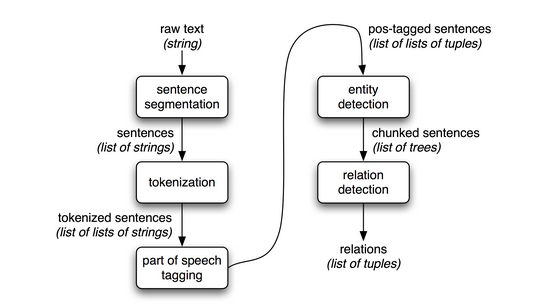
\includegraphics[scale=0.4]{images/nltk.png}
\end{figure}
\end{itemize}

\section{ Named Entity Recognation and Classification  NERC}
%\Jnote{Please do not number sections by hand.}
The term "Named entity" has been coined in 1996 in "sixth  Message understanding Conference"(MUC-6  R. Grishman and  Sundheim 1996).
%\Jnote{No manual citations, use \textbackslash cite in LaTeX. Also it is not usual to write the conference name, just {``has been coined in 1996 by \textbackslash cite{\}''}
Entity can be referred as a task, the entity is "named" when it is restricted to one or many rigid designators \citep{sharnagat2014named}, example: persons,location ,product are the named entities.

Based on the classification of Standard Generalizes Markup Language(SGML) a task can be divided into three subtasks:
\begin{itemize}
\item ENAMEX: location,product,country ,organization
\item NUMEX : percentage,quantity 
\item TIMEX : time, date
\end{itemize}

The entities from different reports.
For extracting entities in a report there are different models which can be used:

\section*{2.1.1. Hidden Markov Model}
This model is based on Bayesian probability inference which has been initiated in 18th century. HMM is the earliest applied model for Natural Entities Recognition for English language.The way needed task to be performed is to find the most likely sequence of tagged names(TN) given a sequence of words(SW).
\begin{align}
P(TN|SW) & = \frac{P(SW|TN)P(TN)}{P(SW)}\label{eq2.0.1}
\end{align}
The equation  \eqref{eq2.0.1} is conditional probability, $P(TN|SW)$ can be  called posterior and it is  the probability of an event Sequence of word occurring given Tagged names has observed. 
$P(SW|TN)$ is also called likelihood means it is the probability of observing the sequence of words(SW) when the given hypothesis tagged name(TN) is true. on another hand P(TN) doesn't depend on the evidences,P(TN) is called prior means that it is true even if there is no given evidence at all(masters thesis).We can be ignored P(SW) and the remaining objective is to maximise the probability of getting the sequence of tagged names when sequence of words is given.
%\Jnote{``The above sentence is true.'' Delete that.}
%\Jnote{s/there is a permission to say/we can ignore}
%\Jnote{s/remaining purpose/remaining objective}
\begin{align}
Max\left[P(TN|SW)\right] \label{eq2.0.2}
\end{align}
From the equation  \eqref{eq2.0.2} of the maximization , the following estimation can be made
\begin{align}
P(TN){\approx} \prod_{i=1}^{n} P({TN}_{i}|{TN}_{i-1}) \label{2.0.3}
\end{align}
Where ${TN}_{i}$ is a tag in the sequence of names (TN) , for the likelihood probability can be estimated as 
\begin{align}
P(SW|TN){\approx} \prod_{i=1}^{n} P({SW}_{i}|{TN}_{i})\label{2.0.4}
\end{align}
%\Jnote{There is a typo in formula above.
%  Try explaining better what those estimates mean, something like
%  ``we make a simplifying assumption that the tags occur independently
%  from each other''.}
The above estimations was for a small sequence where ${TN}_{i}$ is a tag in the sequence of names (TN) and ${SW}_{i}$ is a tag at index i in a sequence words (SW).For the large training corpus , the needed step is estimate based on the number of times the tag occurs and the position of the tag in a given corpus.
\begin{align}
P(T_{i}|T_{i-1}) = \frac{K(T_{i-1},T_{i})}{K(T_{i-1})}\label{2.0.5}
\end{align}
Based on the training corpus, $K(T_{i-1},T_{i})$ is referred as a how many times the tag $T_{i}$ occurs after the tag $T_{i-1}$. in the corpus , $K(T_{i-1})$ is considered as the number of occurrences for the tag $T_{i-1}$.

Therefore the estimation can be performed as follow:
\begin{align}
P(C_{i}|T_{i}) =  \frac{K(T_{i},C_{i})}{K(T_{i})} \label{2.0.6}
\end{align}
From the equation \eqref{2.0.6} , the term $K(T_{i},C_{i})$  is referred as the sum of the times that a word "$C_{i}$" has a tag $T_{i}$in the training corpus.
The process of computing the posterior using the above steps is called Markov model.

%\Jnote{This is a beginning of a good explanation, but you need to rewrite to correct language mistakes and clarify some points.}

\section*{2.1.1.1. Advantages of Hidden Markov Model}
%\Jnote{There is no need for a separate section, just put it in another   paragraph.}

It is one of the most powerful statistical and machine learning (ML) techniques in modelling and high qualified in entities extraction.When the researcher is willing to train new data, HMM is very robust and efficient in computations.
\section*{2.1.1.2. Disadvantages of Hidden Markov Model}
One of the limitations of HMM is that the researcher must have the notion of model topology and statistical techniques on how to deal with large amount of training data.
\section*{2.1.2.  Supporting Vector Machine based model(To be edited for non linear data)}
This model has an aims of classifying the named entities by using the linear support vector machine which separate input train documents into two categories, a document must be categorized as either positive or negative and be represented in two dimensional graph.
%\Jnote{You will have many dimensions, not just two}
Hyperplane is for separating train documents based on their categories and "w" is a weight vector  which is perperndicul to hyperplane is represented by the following equation: 
\begin{align}
w.x- b = 0 \label{2.0.7}
\end{align}
\begin{figure}[hbtp]
\caption{SVM in hyperplane representation}
\centering
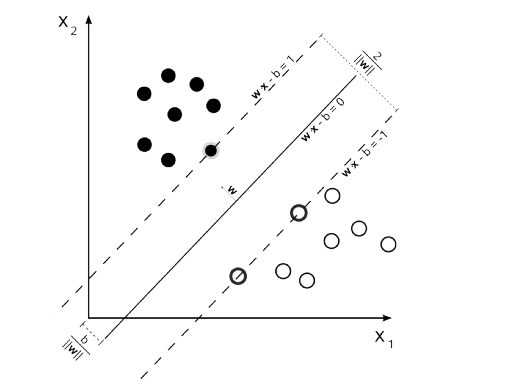
\includegraphics[scale=.7]{images/svm.png}
\end{figure}

 

From the \eqref{2.0.7}, the offset of the hyperplane is $ \frac{b}{\parallel  w \parallel} $

The target is to maximize the the margin between the the points which represent two categories.remember that the vectors which pass through each of the point representative is perpendicular to the w , suppose that there will be an imaginary line which join two borders points $ h_{-}$ and $ h_{+}$.
%\Jnote{I didn't understand this explanation.}
Supporting vectors which are demonstrated by the dashed lines on the figure above  are formed by :
\begin{align}
w.x- b & = 1 \label{2.0.8} \quad \quad \quad  \text{and also } \\
w.x- b & = -1 \label{2.0.9}
\end{align}
There are many algorithms with different approaches to optimization problems but all tends to the same solution says that minimize $\textbackslash w \textbackslash$ automatically maximize the margin between $ h_{-}$ and $ h_{+}$ where the boundary is a half way.
%\Jnote{Don't use \textbackslash parallel for norm, instead use \textbackslash\textbar}
Now,add another constraint for each document category from the equations \eqref{2.0.8} and \eqref{2.0.9}, in order to hit the target
\begin{align}
w.x- b & \geq     1 \label{2.0.8} \quad \quad \quad  \text{and also } \\
w.x- b & \leq -1 \label{2.0.9}
\end{align}
%\Jnote{Again, I didn't really understand this part.}


\section*{2.1.2.1 Disadvantages of SVM} 

The classification of particular documents is not easy to be performed by SVM without destroying the constructed weights  but with hand-written rule model. the machine learning prefers to use the decision tree procedure than SVM. in addition the decision tree has a detailed boolean-like  model which is more popular to user.

\section*{Overview of rule/patern based systems hand-written rule,decison tree,bootstracpping and  }

\textit{Hand-written rule}

It is one of the standard approaches of NER and IE,it has been used for extracting the patterns from automated pages such as amazon, NLP is so useful for unstructured humman-written text by delivering  part-of-speech (POS), syntactic parsing and categories of semantic words.

\textit{Rule /pattern based extraction}

Many IE systems uses rule/pattern to extract words and also phrases by looking to the context of those words or based on the their surroundings.\citep{califf2003bottom}.some system decided if the procedure of extracting the words should rely on the meaning of each word independently or on the context of their surroundings in a phrase.
The limitation of this method is that some words do not have a closer mining to their surroundings that is why Patwardhan Siddharth with help of Ellen Rilo  in workshop called "ACL 2006" presented another approach which  was  generating an automated IE system to learn patterns from a large fixed data set  within a specific domain \citep{patwardhan2007effective} 

Our research deals with reports generated through a template, compaired to the work of  \citep{patwardhan2007effective} templates usages is a limitation.

%The purpose of Rule based extraction is to show in the text "Who" did "what" and "How"




\section*{2.1.3. Text classification and Naive Bayes}
It is one of the most important algorithm in text classification by using base rule and bag of words to classify the entities \citep{manning2012information}.The user instead of going through the report and start posing many queries, text classification algorithm transient the need information.
Its aims is to build a function $\theta$ which takes the bag of words and returns the class of sentiment $C$ either positive or negative.

{ \centering{$\theta$}

\centering{$\Updownarrow$}   

\begin{figure}[hbtp]
%\caption{a part of a sample reeport}
\centering
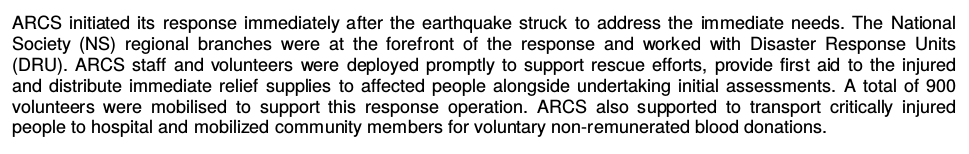
\includegraphics[scale=0.4]{images/report.png}
\end{figure}

{\centering{$\Updownarrow$}}

{\centering{C}}

The procedure is to look for all words and retrieve those which form the subsets.  bag of words are formed after throwing away  all words except the subsets.The use of the function $\theta$  is for  attributing  to each item of the bag of words a sentiment.}

%\section*{2.1.4. Condition Random Field  based model}
%CRF is modeling metho
%
%
%






Information extraction is a combination of segmentation, classification and clustering 





















































































































